\hthree{"Middleware"}\label{sec:middleware}

Bei \ZELIA\ ist eine "Middleware" eine Funktion, die eine bestimmte Signatur hat (siehe Code \ref{code:middlewareSignature}), welche von "express" vor der Handler-Methode des "Controllers" aufgerufen wird. 
Diese benötigt die aus dem NPM-Modul "express" bekannten Parameter:

\begin{itemize}
    \item \textbf{Request-Objekt} ({\ttfamily req}) -- beinhaltet alle Informationen des Requests. Dazu zählen \zb\ die Header, Query-Parameter oder der Body.
    \item \textbf{Response-Objekt} ({\ttfamily res}) -- ermöglicht das Erstellen einer Antwort. Dafür können mit diesem Objekt der Statuscode, die Header und der Body gesetzt werden.
    \item \textbf{Next-Funktion} ({\ttfamily next}) -- muss aufgerufen werden, wenn die Middleware fertig ist, ohne dass dieser die Anfrage durch eine Antwort beendet hat.
\end{itemize}

"Middlewares" können entweder für einzelne Methoden im "Controller", für einzelne "Controller" oder für die gesamte API registriert werden. Soll die Middleware für die gesamte API zur Verfügung stehen, muss diese im App-Konstruktor registriert werden.

\typescript[code:middlewareSignature]{code/APITemplate/middleware.ts}{Signatur einer Middleware}

\hfour{Anwendungsfälle}

Eine "Middleware" könnte zum Beispiel Informationen über die eingehenden "Requests" loggen, damit die Entwickler leichter debuggen können. 
Dabei wird sie im \linebreak App-Konstruktor registriert, um bei jeder Anfrage mitzuloggen. 

\begin{figure}[H]
    \centering
    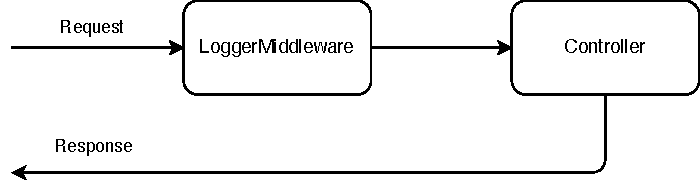
\includegraphics{media/APITemplate/LogMiddleware.svg.pdf}
    \caption{Aufrufreihenfolge der "Middlewares" vor dem "Controller" anhand der "LoggerMiddleware"} 
\end{figure}

\typescript{code/APITemplate/loggerMiddleware.ts}{Beispiel der "LoggerMiddleware"}

"Middlewares" können auch benutzt werden, um den Benutzer beim "Request" zu \mbox{authentifizieren}.
Dabei wird in der "Middleware" geprüft, ob der Nutzer auf diesen Endpunkt zugreifen darf. Wenn ja, wird die "Next"-Funktion aufgerufen, um die nächste "Middleware" bzw. die Handler-Methode des "Controllers" aufzurufen. Wenn nicht, wird mittels des "Response"-Objektes eine "Unauthorised-Response" geschickt.

Wenn die "Logger"-"Middleware" in der App-Klasse und die "Authentication"-"Middleware" in einem "Controller" registriert sind, wird bei einer Anfrage auf diesen "Controller" zunächst die "Logger"-"Middleware" ausgeführt. Danach wird in der "Authentication"-"Middleware" geprüft, ob der Nutzer berechtigt ist, auf diesen Endpunkt zuzugreifen. Wenn ja, wird die "Next"-Funktion aufgerufen, um die nächste "Middleware" bzw. die Handler-Methode des "Controllers" aufzurufen. Wenn nicht, wird mittels des "Response"-Objektes eine "Unauthorised-Response" geschickt (siehe Abbildung \ref{fig:authMiddleware}).

\begin{figure}[H]
    \centering
    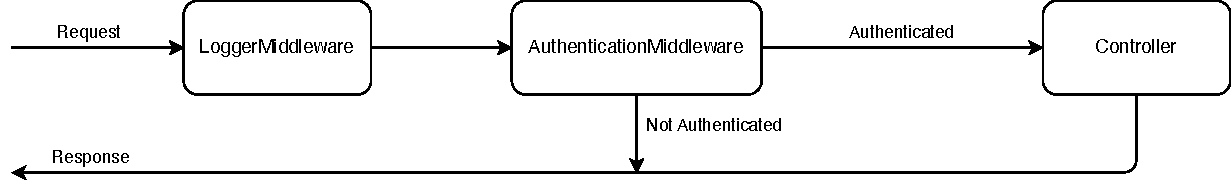
\includegraphics[width=15cm]{media/APITemplate/AuthMiddleware.svg.pdf}
    \caption{Aufrufreihenfolge der "Middlewares" vor dem "Controller" anhand der "LoggerMiddleware" und der "AuthenticationMiddleware" } 
    \label{fig:authMiddleware}
\end{figure}

\typescript{code/APITemplate/authenticationMiddleware.ts}{Beispiel der "Authentication"-"Middleware" }
